\section{Methodology}

\subsection{Brief Simulation Description}

Before listing the input parameters, we briefly describe the simulation again.

This program is meant to simulate proton-proton collisions at very high energies. In particular, this model implements the scattering of quarks at leading-order via an intermediate $Z$-boson or photon. The Feynman diagram for this process is given in Figure~\ref{fig:main-diagram}.

\begin{figure}[ht]
  \centering

  \begin{tikzpicture}
    \begin{feynman}[large]
      \vertex (a);
      \vertex [above left = of a] (i1) {$q$};
      \vertex [below left = of a] (i2) {$\bar{q}$};
      \vertex [right of = a] (b);
      \vertex [above right = of b] (f1) {$\ell$};
      \vertex [below right = of b] (f2) {$\bar{\ell}$};

      \diagram* {
        (i1) -- [fermion] (a) -- [photon, edge label=$Z/\gamma^*$] (b) -- [fermion] (f1),
        (i2) -- [anti fermion] (a),
        (b) -- [anti fermion] (f2)
      };
    \end{feynman}
  \end{tikzpicture}
  
  \caption{Feynman diagram for $pp \rightarrow Z/\gamma^* \rightarrow \ell\ell$ at leading order.}
  \label{fig:main-diagram}
\end{figure}


There are two components to the simulation: the hard scattering process and the parton showering. The hard scattering process consists of a Monte Carlo alrogithm which randomly generates phase space points (such as angle of the collision) and computes the total cross section of the interaction. This cross section essentially corresponds to a probability for the reaction to occur. With this cross section, we can then generate events by randomly generating numbers and accepting an event corresponding to the ratio of the randomly generated event's cross section to the overall maximum obtained cross section during the Monte Carlo part. What we are left with, then, is a selection of events that are normally distributed according to their cross sectional weight.

The second part is the parton showering. This is done by taking a quark at some initial energy and using the Sudakov form factor to evolve the quark to lower and lower energy scales. The Sudakov factor essentially calculates the probability that the quark \textit{doesn't} emit a gluon from the initial scale $t_0$ to final scale $t$. By randomly generating numbers to determine the scale $t$ at which the quark will emit a gluon, we can have the quark emit a gluon at that scale. This is done until the quark has too little energy to continue emitting gluons.

\subsection{Input/Variable Parameters}

Here, we list all of the input parameters that can be configured prior to running the hard scattering process:

\begin{itemize}
\item \textbf{PDF Set}: The collision is a proton-proton collision, but we calculate sub-processes of the proton's constituent quarks. PDFs contain information related to the quark content of the proton, allowing us to correctly compute the cross section for the total interaction.
\item \textbf{ECM}: The Energy in the Center-of-Mass frame is essentially twice the energy of each proton. Higher energy collisions give rise to different cross section values, and hence a different distribution of final events.
\item \textbf{MinCutoffEnergy}: When randomly generating phase space points, the energy of the quark is generated. A quark with sufficiently low energy would cause computational problems (think of a division-by-zero issue), so this determines that cutoff to avoid those problems. Additionally, there is a physical lower limit before the quarks are no longer ``free'', meaning they no longer are capable of being present in an interaction like this. Such an energy is usually $\mathcal{O}(\qty{1}{\giga\electronvolt})$, but is defaulted as a higher number to be extra safe.
\item \textbf{TransformationMass/TransformationWidth}: These are purely intermediate calculation parameters with no physical significance. They are used in the change-of-variable transformation for one of the integrals in the cross section calculation to make the Monte Carlo algorithm more efficient. They are initially chosen to be the same as the minimum cutoff energy, and shouldn't go below it, but can in principle be made arbitrarily higher.
\end{itemize}

For the parton showering part of the simulation, the configurable parameters are:

\begin{itemize}
\item \textbf{InitialEnergy}: This is the initial energy that the quark contains before it begins emitting gluons. It is initially chosen to be $\mathcal{O}(\qty{1}{\tera\electronvolt})$, as that is usually the characteristic energy of a subprocess from an initial $\qty{14}{\tera\electronvolt}$ proton-proton interaction like that done for the hard scattering process.
\item \textbf{FixedScale}: The value/strength of the coupling between quarks and gluons is called the coupling ``constant'' but technically varies slightly. The slight variations are considered higher-order effects, meaning that at leading order we typically leave it as a true constant. However, there is the possibility to compute it on the fly at each characteristic energy scale during the evolution, which would, in principle, give more accuracy. This is a Yes/No option.
\item \textbf{EvolutionEnergyCutoff}: This is analogous to the \textbf{MinCutoffEnergy} for the hard scattering process. At this energy (and below), quarks would no longer be likely to emit gluons; rather, they would bind to other quarks to create \textit{hadrons} (like a proton). It also serves to avoid some computational issues like division-by-zero.
\end{itemize}




\subsection{Variance Plan}

All of the above parameters are going to be tested individually, since they, in principle, are all related in the output of the final events. If multiple were to be varied in any given run, it would be very challenging to make a distinction between the effects of any of the varied parameters.

For the hard scattering process, the following is how I plan to vary each parameter:

\begin{itemize}
\item \textbf{PDF Sets}: I plan to test three PDF sets that should all be relatively good. In general, PDF sets can focus more heavily on corrections to only certain areas, but there are many that are general and don't bias one way or the other. The three pdf sets are: \textit{cteq6l1}, \textit{CT18NNLO}, \textit{NNPDF30-nlo-as-0121}. The first two are from the CTEQ collaboration, with the very first being a highly popular PDF set made almost 3 decades ago now but still being used in many places for compatibility. The second is a far more recent set containing many more higher order effects. The last is a similar set from the NNPDF collaboration. It isn't possible to predict exactly the influence of changing the PDF sets, because in general including higher order effects doesn't have to strictly increase or decrease the value of outputs, but it will be helpful nonetheless to see what indeed does happen to the cross section and event distribution.
\item \textbf{ECM}: This parameter will be varied from $\qty{8}{\tera\electronvolt}$ to $\qty{20}{\tera\electronvolt}$. Any lower would be useless since most colliders nowadays do not access such a low energy. Results wouldn't be inaccurate necessarily, they just wouldn't be useful to compare to current data with. The upper end follows a similar rationale -- the current ECM in CERN is $\qty{14}{\tera\electronvolt}$, so this gives a $\pm\qty{6}{\tera\electronvolt}$ range to work with.
\item \textbf{MinCutoffEnergy}: This will be varied down to $\qty{20}{\giga\electronvolt}$ to $\qty{200}{\giga\electronvolt}$. As mentioned above, any lower and we incur computational issues as well as accessing energies that are otherwise highly unlikely to actually occur. Any higher than the upper limit and we are beginning to more severely limit the phase space by ignoring perfectly likely events.
\item \textbf{TransformationMass/Width}: These will be varied from $\qty{20}{\giga\electronvolt}$ to $\qty{500}{\giga\electronvolt}$, a much higher range than the previous parameter. Again, since there is no particular physical significant to this parameter, this is simply to see how varying this parameter effects computational efficiency.
\end{itemize}

\begin{center}
  \begin{table}[ht]
    \centering
    \begin{tabular}{|c||c|c|c}
      \hline
      Variable & Range & Expected Output \\ \hline
      $E_{CM}$ & $[\qty{8}{\tera\electronvolt},\qty{20}{\tera\electronvolt}]$ & Pushing of output energy/momentum distributions right. \\ \hline
      $E_{\mathrm{min}}$ & $[\qty{20}{\giga\electronvolt},\qty{200}{\tera\electronvolt}]$ & Invalid results on the lower end; increased uncertainty on the higher end \\ \hline
      $E_{\mathrm{tr}}/\Gamma_{\mathrm{tr}}$ & $[\qty{20}{\giga\electronvolt},\qty{500}{\tera\electronvolt}]$ & Same as for $E_{\mathrm{min}}$ but more extreme \\ \hline
    \end{tabular}
    \caption{Expected outcomes for changing of the hard scattering input parameters.}
    \label{tbl:hard-scattering-vars}
  \end{table}
\end{center}

A table summarizing this information is given in Table~\ref{tbl:hard-scattering-vars}. To elaborate a little further on the expected outcome for $E_{\mathrm{CM}}$, since we are pushing the overall center-of-mass energy up, this would generally increase the cross section for the process, meaning that higher-energy events are more likely. Because of this the distribution of energy/momentum (transverse momentum, $p_T$ in particular) is likely to shift rightwards.

In terms of how this will be shown in the Results section, since the cross section is a single number, we can vary the parameters nearly continuously and display a single curve. However, the other output from the simulation that can in principle be impacted by varying these parameters is the distribution of kinematics from the generated events. Since this is an entire distribution rather than a single number, we will only pick 2-3 points from each range and display the resulting distributions overlayed, as I believe this is the easiest way to visualize the results.

Now, for the parton showering process, the following is how I plan to vary each parameter:

\begin{itemize}
\item \textbf{InitialEnergy}: This will vary from $\qty{500}{\giga\electronvolt}$ to $\qty{7}{\tera\electronvolt}$. The lower range is already quite low for a reaction involving quarks, but it will serve well to test the model. The upper limit is similarly unlikely to actually happen, but serves as a good test.
\item \textbf{FixedScale}: This is simply a yes or no, so it can only take two values. The \textbf{InitialEnergy} and \textbf{EvolutionEnergyCutoff} will be varied through their full ranges twice, once with this parameter set to Yes, once with it set to No.
\item \textbf{EvolutionEnergyCutoff}: This parameter will have a very small range in which it is varied, since it essentially corresponds to the fixed cutoff at which QCD, the regime in which calculations are done, becomes ineffective due to quarks not wanting to emit gluons (it is more complicated than this, but it gets the point across). Any lower and results are not physical at all, and any higher we miss out on genuine possible reactions that could occur. Therefore, this will only be varied from $\qty{1}{\giga\electronvolt}$ to $\qty{10}{\giga\electronvolt}$.
\end{itemize}


\begin{center}
  \begin{table}[ht]
    \centering
    \begin{tabular}{|c||c|c|c}
      \hline
      Variable & Range & Expected Output \\ \hline
      $t_0$ & $[\qty{500}{\giga\electronvolt},\qty{7}{\tera\electronvolt}]$ & Influence of output distributions on lower end. \\ \hline
      Scale & Yes/No & Reduced statistical uncertainty. \\ \hline
      $t_f$ & $[\qty{1}{\giga\electronvolt},\qty{10}{\tera\electronvolt}]$ & Same as $t_0$. \\ \hline
    \end{tabular}
    \caption{Expected outcomes for changing of the parton showering input parameters.}
    \label{tbl:parton-showering-vars}
  \end{table}
\end{center}

A summary is given in Table~\ref{tbl:parton-showering-vars}. It is worth noting that in this case the expected outcomes are a simplistic. That is because the other effects apart from the more obvious ones listed are hard to gauge. In general anyway, physics at this scale is inherently intuitive, so this is really all I am able to say. Further, unlike the hard scattering process which outputted both the cross section, a single number, and the kinematic distributions of the output events, the parton showering process only contains the latter. Therefore, similar to the hard scattering case, I'll only pick a few points from each interval for each variable.


\subsection{Scenario Analysis}

From my understanding of scenarios, as they are used in the context of this assignment, I believe that my model is incompatible with them. My reasoning ties back to what has been described about my model's specifics previously. In particular, the nature of my model simply doesn't allow for ``optimistic'' or ``pessimistic'' or any type of scenario at all, because there is nothing necessarily good or bad to expect. The example in the assignment gives things like higher or lower demand in the markets, which have good/bad real-world consequences. My model, on the other hand, is a model of a process in quantum physics. The behavior and mathematics the underpin it very tightly bind the process to behave in only a specific way, a part of which I attempt to capture with my model/simulation.

What I am trying to convey is that there are only two concrete scenarios for my simulation: either I follow the theorems and implement what is known in the current literature and accurately simulate what happens in the real world, or I violate any one of the dozens of theorems and assumptions in place that make modeling/simulating the model possible in the first place. Further, as a model that doesn't necessarily have the same effects directly on the everyday lives of people as traffic models or economical models, it is significantly harder to quantify what is even ``optimistic'' or ``pessimistic'' in the first place. The physics either occurs as expected, or doesn't -- there's nothing else to it.

Therefore, I believe that it is not beneficial (or possible, really, without really stretching some things) to define scenarios and carry out this particular part of the procedure. I feel that, in the previous section, I have done as much as I can in terms of validating how the model performs under the changing of the various input parameters. I have also done my best to tie the changing of the input parameters to their physical interpretation in order to try and match at least some of the requirements of this section.



\section{Results}


\subsection{Hard Process Variables}

\begin{figure}[ht]
  \centering
  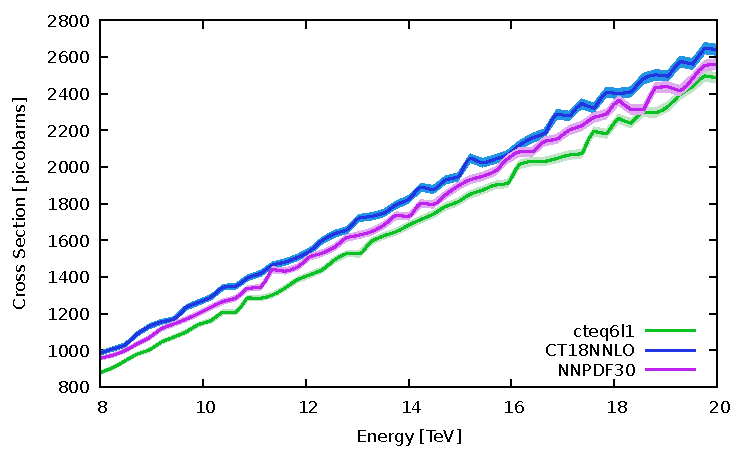
\includegraphics[width=0.7\textwidth]{./res/gfx/xs.pdf}
  \caption{Cross section dependence on center-of-mass energy for the three different candidate PDF sets.}
  \label{fig:ecm}
\end{figure}

Figure~\ref{fig:ecm} contains the curves depicting the dependence of the cross section on the center-of-mass energy of the main proton-proton collision, where the shaded region indicates the error. Importantly, for most other results we fix the number of iterations of the Monte Carlo iterations to be one million, but in this instance we drop it by a factor of 10 in order to increase speed. As we expect, the cross section grows monotonically with the ECM. Additionally, we can tell that the most accurate PDF sets increase the total value of the cross section due to the fact that they contain more corrections to the main process. Overall, the model performs well and as expected in this area.


\begin{figure}[ht]
  \centering
  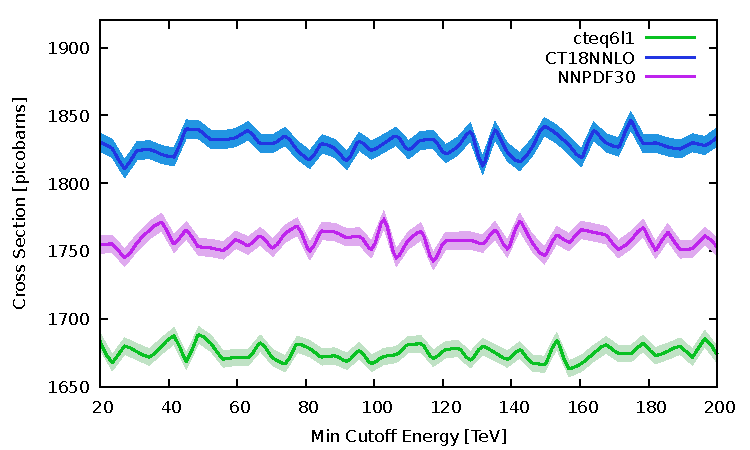
\includegraphics[width=0.45\textwidth]{./res/gfx/cutoff.pdf}
  %\includegraphics[width=0.45\textwidth]{./res/gfx/trans-energy.pdf} 
  \caption{Cross section dependence on the minimum cutoff energy (left) and transformed mass/width (right) for the three different candidate PDF sets.}
  \label{fig:cutoff-trans}
\end{figure}

Figure~\ref{fig:cutoff-trans} contains similar curves as Fig.~\ref{fig:ecm} but for the minimum cutoff energy and transformed mass/width. The $E_{\mathrm{CM}}$ was kept fixed at $\qty{14}{\tera\electronvolt}$. Interestingly, we still note that the more accurate PDF sets give larger results, but unexpectedly the two variables seem to have very little effect on the actual value of the cross section, though it does vary relatively widely. This is actually a very good thing, especially for the transformation mass/width, because that variable is an intermediate variable present only for calculational purposes, meaning that it \textit{shouldn't} have any effect on the cross section. Further, while the minimum cutoff energy technically has physical implications, we don't vary it low enough for those physical effects to manifest, meaning it also shouldn't have an effect.

We next show the dependence of the distributions for the events that were generated after varying the ECM. We know now that the changing of the intermediate calculation variables does not have a noticable effect on the cross section, which is the fundamental quantity influencing the generation of events via the hit-or-miss method. Therefore, we will not show their effect. Further, the energy of the output events is the only distribution which we will show, since it is has the most clear physical implications.

\begin{figure}[ht]
  \centering
  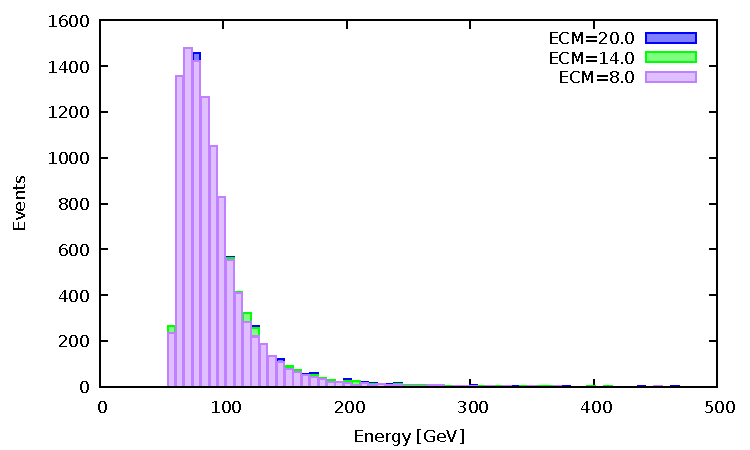
\includegraphics[width=0.7\textwidth]{./res/gfx/Q.pdf}
  \caption{$Q$ distributions after varying the center of mass energy.}
  \label{fig:q-dist}
\end{figure}

This is done in Figure~\ref{fig:q-dist}. It is surprisingly hard to notice, but the lower energy distribution has a sharper peak at a lower energy, while the higher energy distribution has a slightly more spread out peak but is noticeably shifted to the right. The extent to which it is shifted is much smaller than I would have expected, however, the fact that it is still obviously occurring means that the model is performing correctly. More work will be done, though, to look into whether it should be shifted as little as it is.

\subsection{Parton Showering}

Like mentioned previously, the parton showering process only spits out some distributions of the kinematics from the final state events, rather than any single numbers like the hard scattering part of the simulation. Also, similarly, some of these variables are intermediate calculation variables or have a less obviously physical significance, with the exception of the transverse momentum $p_T$.
\begin{figure}[ht]
  \centering
  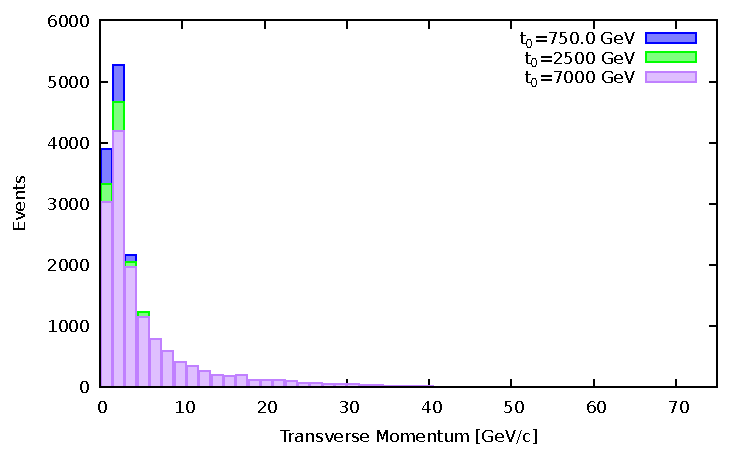
\includegraphics[width=0.45\textwidth]{./res/gfx/pt-fixed.pdf}
  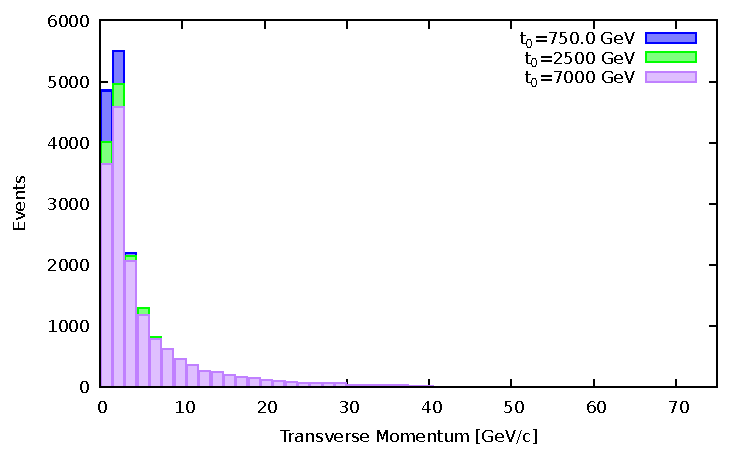
\includegraphics[width=0.45\textwidth]{./res/gfx/pt-variable.pdf}
  \caption{$p_T$ distributions for the generated parton showering events by varying the initial evolution energy for a fixed scale for the coupling (left) and a variable scale for the coupling (right).}
  \label{fig:pt-dist}
\end{figure}

Figure~\ref{pt-dist} contains two plots containing the output transverse momentum $p_T$ distributions for the generated parton showering events. On the left, the scale for the coupling $\alpha_s$ is kept fixed (and hence its value is also constant), and on the right, it is varied throughout each evolution.

The results here are a little bit more easy to see, and are as expected if we again consider the definition of the Sudakov factor. This factor determined the probability that the quark does \textit{not} emit a gluon from some initial scale $t_0$ to a final scale $t$. This means that for a particular evolution starting at a $t_0$ which higher compared to another at $t_0'$, it is essentially just as probable for the former evolution to emit a quark at a $t$ which is higher compared to the latter evolution at $t'$. The point is that it is more likely to emit gluons at a higher evolution scale when starting the evolution itself at a higher value (phrasing it this way makes it seem very intuitive, but it helps to have a mathematical grasp).

This is reflected in the plots since we see that the distributions corresponding to higher initial evolution scales are shifted to the right, corresponding to the fact that higher $p_T$ events are more likely. Evidently, the model is performing as expected in this regard. Another thing that we notice is that varying the coupling vs. keeping it fixed seems to have very little effect. This is expected: the fixed coupling is chosen to be at the scale of half of the initial evolution scale, meaning that, on average, it \textit{roughly} captures what the variable coupling would capture. Only super minor effects would matter, and those are impossible to tell in the graph. Further, the ``additional effects'' are only NLO effects, not NNLO or N$^3$LO (the order to which corrections to the couplings are known), meaning they are already very small.

\begin{figure}[ht]
  \centering
  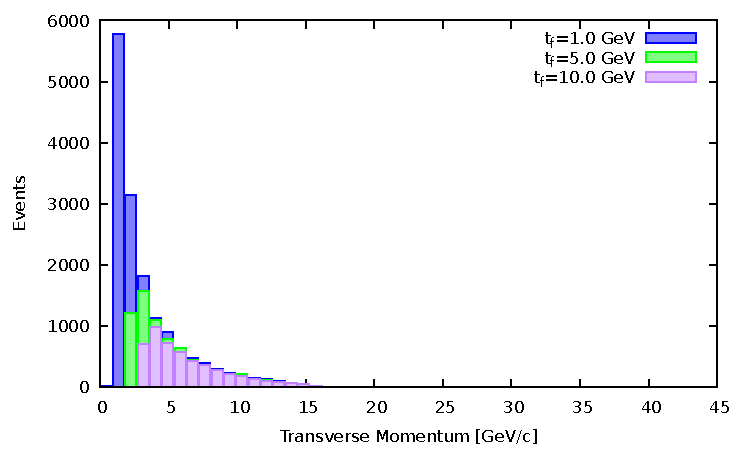
\includegraphics[width=0.45\textwidth]{./res/gfx/pt2-fixed.pdf}
  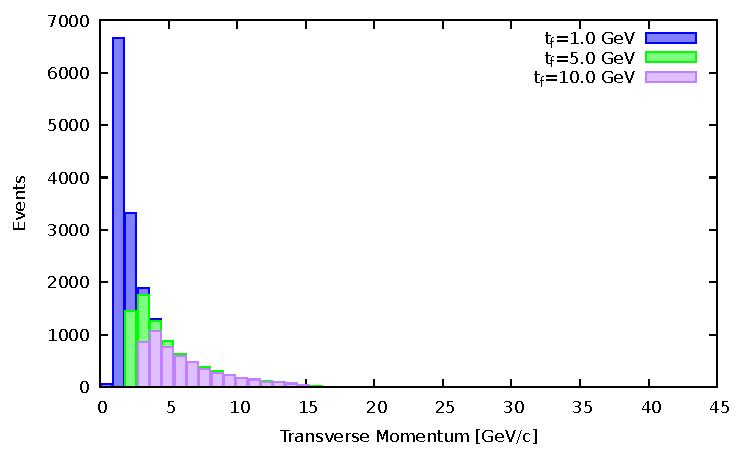
\includegraphics[width=0.45\textwidth]{./res/gfx/pt2-variable.pdf}
  \caption{$p_T$ distributions for the generated parton showering events by varying the evolution cutoff energy for a fixed scale for the coupling (left) and a variable scale for the coupling (right).}
  \label{fig:pt-dist2}
\end{figure}

In Figure~\ref{fig:pt-dist2}, I have done the same but this time by varying the final cutoff energy. This had the most notable effect of dramatically reducing the number of emissions that were generated by the end for the cases with higher cutoff. Further, the shape of each distribution is essentially identical, which makes sense. This is exactly as expected and shows further that the model works as expected.



%%% Local Variables:
%%% mode: LaTeX
%%% TeX-master: "../../FinalMilestone"
%%% End:
